\chapter{基于模糊逻辑的异构Hadoop集群配置优化}
\label{chapter:hadoop}

\section{引言}

随着云计算的发展,大规模的数据中心越来越多,越来越多的公司需要管理这些大量
的服务器。这些由廉价个人计算机组成的集群由于设备淘汰率高,更换设备的频
率也更高,从而使得集群内部大量存在着异构的服务器。这些异构的服务器有些
拥有不同的硬件配置,有些运行着不同版本的操作系统,有些甚至可能运行在不
同体系结构下。那么在每次更新或者升级数据中心之后,如何动态的对Hadoop集
群进行重新配置以使达到最佳的执行效率就成为数据中心维护人员的一项重要工
作。

Hadoop项目\cite{hadoopproject}包含了Apache基金会下的一系列开源项目:
MapReduce、HDFS、HBase\cite{hbaseproject}、Hive\cite{hiveproject}等。由于它的完整性和高可用性,一出现就成为了工业界和学术界进行大规模计算研究和应用的标准平台。大量的公司(如\ref{table:hadoopcluster}所示)内部往往运行着数以万计的服务器组成的Hadoop集
群来完成各种各样的工作。

\begin{table}[h!]\small
  \caption{典型的Hadoop集群的规模\cite{hadooppowerby}}
  \label{table:hadoopcluster}
  \centering
  \begin{tabular}{|c|c|}
    \hline
    \textit{Institution} & \textit{Scale} \\
    \hline
    Ebay & 532节点,4256核心\\
    \hline
    Facebook & 1100/300节点,8800/2400核心\\
    \hline
    百度 & 2000节点,超过8000核心\\
    \hline
    Yahoo! & 4000节点,超过16000核心\\
    \hline
    ... &  ..., ...\\
    \hline
  \end{tabular}
\end{table}

然而Hadoop本身的对集群配置的功能非常弱,配置往往只能在安装时进行
一次配置,之后所有的配置都通过同步的方式传输到所有节点中,并在启动后开
始起作用;如果管理员希望在Hadoop集群运行的过程中修改某些参数,那么只能要求集群
的使用人员在提交任务的时候以命令行参数的形式将新的参数传入Hadoop。但是
这种方法只能修改整个Hadoop可配置参数集中少量的部分。如果希望对别的参数
进行修改则需要重启整个集群,这在大规模的生产环境中是不可以接受的。

除此之外,Hadoop本身作为一个复杂的分布式系统软件,其中包含了大量的可配
置参数,比如版本0.19.2中包括了大约170个配置参数,而这些参数中很大一部
分对所部属的Hadoop性能有较大影响。从Hadoop项目的邮件列表中也可以看出,
在日常使用中如何根据自己集群中服务器的实际配置选择合适的参数是用户在配
置集群时面临的主要问题,而现有的解决方案则是通过一些\textit{艺术化}的指导原则
来进行的\cite{hadooptuning},比如:\textit{如果集群服务器数目较大,应该将
dfs.namenode.handler.count配置更大的值
\cite{hadoopconfexample}}。这种指导性的配置方法显然不适合大规模的集群
管理,特别是当集群中存在异构服务器的情况下。


在本研究课题中,我们使用模糊逻辑的算法,以正在运行Hadoop系统的异构集
群中服务器的各种硬件参数作为模糊输入,设计并实现了一个对Hadoop异构集群进行自动配置的工具。该工具在集群运行的过程中收集
各种运行状态信息,并且根据这些历史数据进行模糊分析。通过模糊逻辑的
方案进行动态参数配置改变了传统Hadoop集群的配置方法,将过去优化参数的方
法转变成了优化规则的方法。而相比较优化参数,优化规则更能够适应
不同的部署环境,更加具有通用性。实验证明,本方法不仅仅降低了Hadoop异构
集群的维护成本,而且极大的提高了任务的执行效率,进一步提高了Hadoop集群的
速率。

\section{相关背景介绍}

\subsection{模糊逻辑}
模糊逻辑由Berkeley大学的L.A.Zadeh与1965年引入的一种基于模糊集合论对布
尔逻辑的扩展理论。首先我们简单描述一下模糊集合。在集合论中,我们称一个
元素是否属于某集合是确定的,也就是说它要么属于,要么不属于,此为是非
二元判断,不过在模糊逻辑中对于元素对集合的从属关系却可以描述为
部分属于集合。并且元素属于集合的程度用可以隶属度(likelyhood)来描述。隶
属度函数是一个0-1之间的集合成员关系值,在自然语言中,通常可以被描述成
为\textit{稍微},\textit{非常}等概念。常见的隶属度函数如:三角隶属度函数、梯形隶属
度函数和高斯隶属度函数等。

与布尔逻辑类似,模糊逻辑也定义了一系列逻辑操作:IF/THEN、AND、OR、和
NOT等。其中AND,OR,NOT被称为Zadeh运算符\cite{klir1995fuzzy},它们的定义如公式
\ref{equa:zadeh}所示:
\begin{equation}
  \label{equa:zadeh}
  \begin{split}
    NOT\quad x = (1 - truth(x))\\
    x\quad AND\quad y = minimum(truth(x), truth(y))\\
    x\quad OR\quad y = maximum(truth(x), truth(y))
  \end{split}
\end{equation}
而IF/ELSE规则相比较布尔逻辑也有所不同,它的IF需要根据元素对多个模糊子
集的隶属度大小来最终判断是否属于某一个集合。

模糊逻辑作为不确定推理的一种,在人工智能中具有非常重要的意义,特别对于
复杂的工控和专家系统来说,它的效果非常好。对于复杂的Hadoop集群的自动配
置来说,模糊推理是一个可行的方案,主要原因在于影响Hadoop集群的参数众多
且关联性强,无法建立一个准确的数学模型来描述。

\subsection{Hadoop参数分析}

Hadoop 0.19.2中共提供了170+个可配置的参数,这些参数中大部分是有关使系统
能够正常工作的配置,比如NameNode的端口配置,ip配置等等,在本文中我们对
于这种不需要改变,并且不会影响到集群性能的配置不予考虑,我们主要分析的
是那些对系统性能会产生较大影响的参数,经过分析共有超过70个此类参数。我
们按照他们的作用时间将其分为3类:
\begin{enumerate}
  \item 在Hadoop系统启动的时候会读取一系列初始化参数并且存储在每一个服
    务器的Hadoop进程所在的地址空间中,这些参数在Hadoop运行中都不会再次
    读入,如果需要对这些参数进行改变,现有系统的唯一做法是重启Hadoop集
    群。
  \item Hadoop启动之后主要向客户端提供基于HDFS的数据访问功能和基于
    MapReduce的任务执行功能。MapReduce中任务执行的基本单位是Job,Job
    由用户提交的可运行的代码和配置文件组成,Hadoop集群在调度
    MapReduce的Job时会向JobConf中加入系统的配置参数,这些参数会被用
    户建立Job时写入的配置覆盖,通常情况下这些参数会改变任务执行效率。
  \item 参数仅仅在一个Job中的多个Task中起作用。Task是比Job更底层的概念,
    一个Job通常包括两类Task:Map任务和Reduce任务,而且每一类Task在系统
    中都同时运行着多个实例。这些Task运行在服务器上的Task Slot上,而每
    一个slot其实就是一个JVM进行。每一次加载Task执行的时候,系统都会动
    态的加载这些参数。
\end{enumerate}

通过对参数生命周期的分类可以将我们的主要研究目标放入到生命周期为Job的
参数,这些参数与Hadoop的基本组件相关,并且也会对系统性能产生显著的影响,
我们对这些参数进一步细分可以得到如下类型:
\begin{enumerate}
  \item 定义时间类型的参数。这些参数定义了事件发生的最小或者最大时间。
    如果设置的过小,可能会导致系统过早的因为意外而进入所谓的伪失败状态,
    而如果设置过高,则容易导致系统对错误响应不及时。
  \item 定义最大尝试次数。很多参数会定义网络行为中最大尝试次数,重复次
    数的多少通常体现了系统对于容错能力的考量。
  \item 定义系统并发度。并发度包括了网络发送的并发度、任务执行的线程并
    发度、网络接受数据的并发度等等。它们描述了Hadoop集群的能力,特别是
    集群规模扩大的时候,并发度也应该随之提高。
  \item 定义资源使用限额。比如允许map任务在本地内存中缓存数据的上限,
    这些参数定义了系统对硬件资源的占用情况。这些参数跟服务器的硬件资源
    情况、集群的拓扑结构和网络带宽都有非常紧密的关系。
\end{enumerate}

表\ref{table:hadoopvars}展示了Hadoop参数的具体分类情况。

\begin{table}[h]\small
  \caption{Hadoop中参数的统计分析情况}
  \label{table:hadoopvars}
  \centering
  \begin{tabular}{|c|c|c|}
    \hline
    \textit{参数类型} & \textit{相关参数数目} & \textit{典型参数实例}\\
    \hline
    & & fs.checkpoint.period \\
    时间类 &  10 & dfs.df.interval \\
    & & dfs.heartbeat.interval \\
    \hline
    & & \\
    重复次数 & 11 & dfs.replication\\
    & & mapred.map.max.attempts\\
    \hline
    & & \\
    并发类参数 & 14 & io.sort.factor\\
    & & mapreduce.reduce.parallel.copies\\
    \hline
    & & \\
    资源使用类 & 25 & io.sort.mb\\
    & & mapred.child.ulimit\\
    \hline
    & & \\
    其他 & 5 & mapred.jobtracker.taskScheduler\\
    & & \\
    \hline
  \end{tabular}
\end{table}

\subsection{Hadoop参数加载流程}
在介绍Hadoop加载参数之前我们先对Hadoop架构做一个简单的介绍。图
\ref{fig:hadooparch}给出了包括HDFS和MapReduce两个模块的标准Hadoop集群
的架构。主节点上同时运行了\textit{NameNode}和\textit{JobTracker}两个服
务,前者负责为分布式存储系统HDFS提供元数据位置信息,后者为MapReduce任
务执行系统提供任务管理和分配服务。主节点之外的子节点运行着
\textit{DataNode}和\textit{TaskTracker}服务,分别负责数据存储和任务执
行。当Hadoop集群启动的时候,首先会启动主节点,之后向所有的子节点同时发
送启动命令,子节点启动时需要向主节点请求元数据信息。

\begin{figure}[h!]
  \centering
  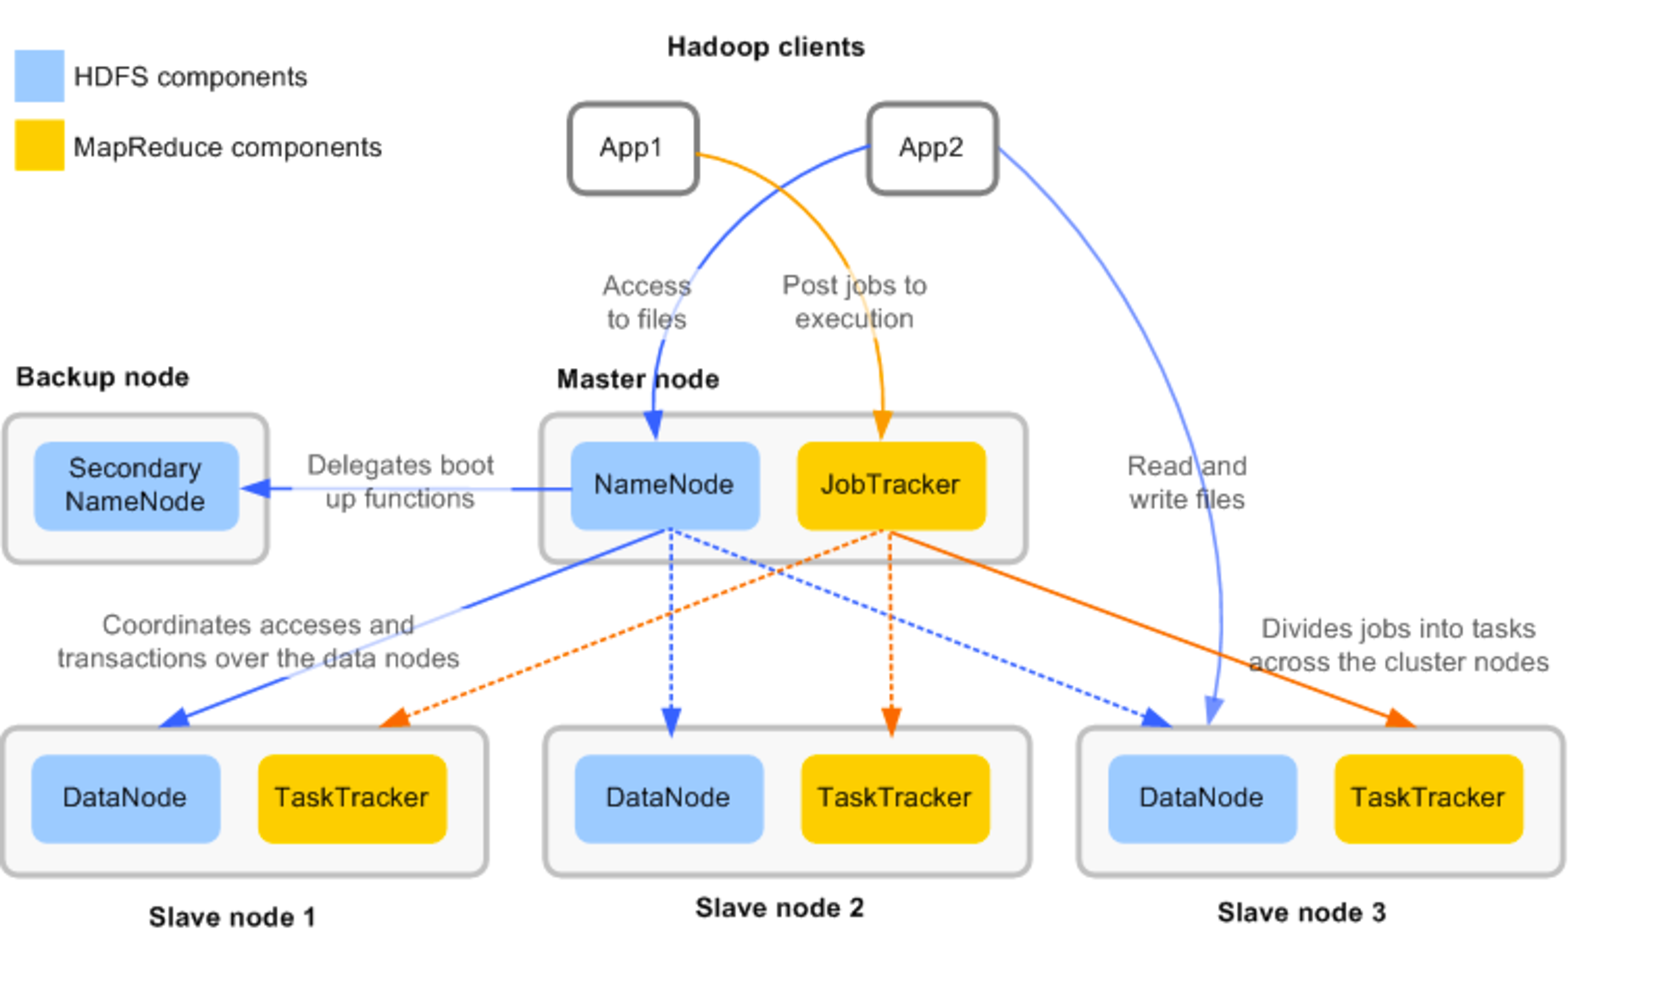
\includegraphics[width=5in]{hadooparch.pdf}
  \caption{Hadoop系统架构}
  \label{fig:hadooparch}
\end{figure}

在这个启动过程中,Hadoop集群中的每一台服务器都需要载入配置参数。这些配
置参数并未维护在一个集中的位置而是存储在每一台服务器上。用户通过手动的
同步操作将配置文件同步到集群的所有服务器上。在每一台服务器上,
\textit{NameNode/DataNode}会首先启动,在本地配置文件在进程空间里生成
一个Configuration对象,紧接着\textit{JobTracker/TaskTracker}启动,生成
JobConf对象。当用户编写一个在Hadoop上运行的MapReduce应用程序的时候,
都需要生成一个JobConf对象并且传递给\textit{JobTracker},此JobConf中的
配置会覆盖掉之前\textit{JobTracker}加载的JobConf对象;最后,当用户的任
务已经提交给\textit{JobTracker},那么集群中的\textit{TaskTracker}都会
通过信条协议向\textit{JobTracker}请求最新的可执行的任务,当获得任务后
将根据其种类(Map任务或Reduce任务)来启动对应的任务,启动的过程中会生成
一个JobConf对象,该对象加载\textit{TaskTracker}本地的配置文件以及用户
提交的JobConf中的数据。

事实上,动态的对于那些已经加载到Hadoop运行时系统中的参数进行修改非常困难。比如参数
\textit{mapred.job.tracker.handler.count}值会决定\textit{JobTracker}中
启动的服务线程的数目。而这些服务线程是在\textit{JobTracker}启动的时候开辟的
线程池。因此即便我们在运行时修改了这个参数,也不会对当前运行中的系统行为产生任何影
响。本文中,对Hadoop集群参数的修改是通过将新生成的参数写入到本地配置文件中,
在下一次启动的时候让Hadoop自动加载实现的。

\section{基于模糊逻辑的配置算法}

\subsection{运行时数据搜集}
我们通过修改Hadoop源码以及分布式的资源检测工具来获得集群的历史运行数据
和所有服务器的硬件指标。并且使用这些信息作为模糊逻辑方案的输入数据来来
计算参数。

\begin{enumerate}
\item 所有节点的Map运行时间的平均值和本节点Map任务执行时间的差
\item 所有节点的Reduce运行平均时间和本节点上Reduce任务执行平均时间差
\item 服务器在执行任务过程中的CPU平均负载
\end{enumerate}

同时我们也需要集群中服务器的硬件指标,包括:
\begin{enumerate}
\item 服务器的CPU频率,以及核心数目。
\item 服务器的内存容量
\item 服务器的硬盘参数
\item 服务器的网络带宽以及接入机架信息
\end{enumerate}
    
\subsection{模糊控制器的实现}
\subsubsection{隶属度函数}
我们使用了混合的隶属度函数来描述Hadoop集群的各种硬件信息,其中包括高斯
型隶属度函数、梯形隶属度函数。梯形隶属度函数能够更好的体现离散输入的特
点,比较适合Hadoop集群中服务器硬件指标数据。

三个隶属度函数分别为:
\begin{equation}
  \label{equa:likelyhoods}
  \begin{split}
    y_{Slow} = gaussmf(x, [sig, c])[sig=2, c=0]\\
    y_{Average} = trapmf(x, [a, b, c, d])[a=3, b=4.5, c=5.5., d=6.2]\\
    y_{Flat} = smf(x, [a, b])[a=4.5, b=9]
  \end{split}
\end{equation}
其中高斯和梯形隶属度函数的表达式如下:
\begin{equation}
  \label{equal:two}
  \begin{split}
    f(x;\sigma,c) = e^{\frac{(x-c)^2}{2\sigma^2}}\\
    f(x;a,b,c,d)=max(min(\frac{x-a}{b-a},1,\frac{d-x}{d-c}),0)
  \end{split}
\end{equation}

实际使用中,服务器CPU频率的变化范围设定为[0,16GHz]。当前主流的CPU为4核,
单核频率2GHz,因此8GHz作为中间值,超过16GHz的单服务器计算能力称为
\textit{很快}的CPU。模糊子集分别为\textit{Slow, Average, Fast},其隶属
度函数在Matlab中可以表示为图\ref{fig:cpulikelyhood}所示。单机CPU频率无
上限,因此使用S型隶属度函数来描述\textit{Fast}。

\begin{figure}[h!]
  \centering
  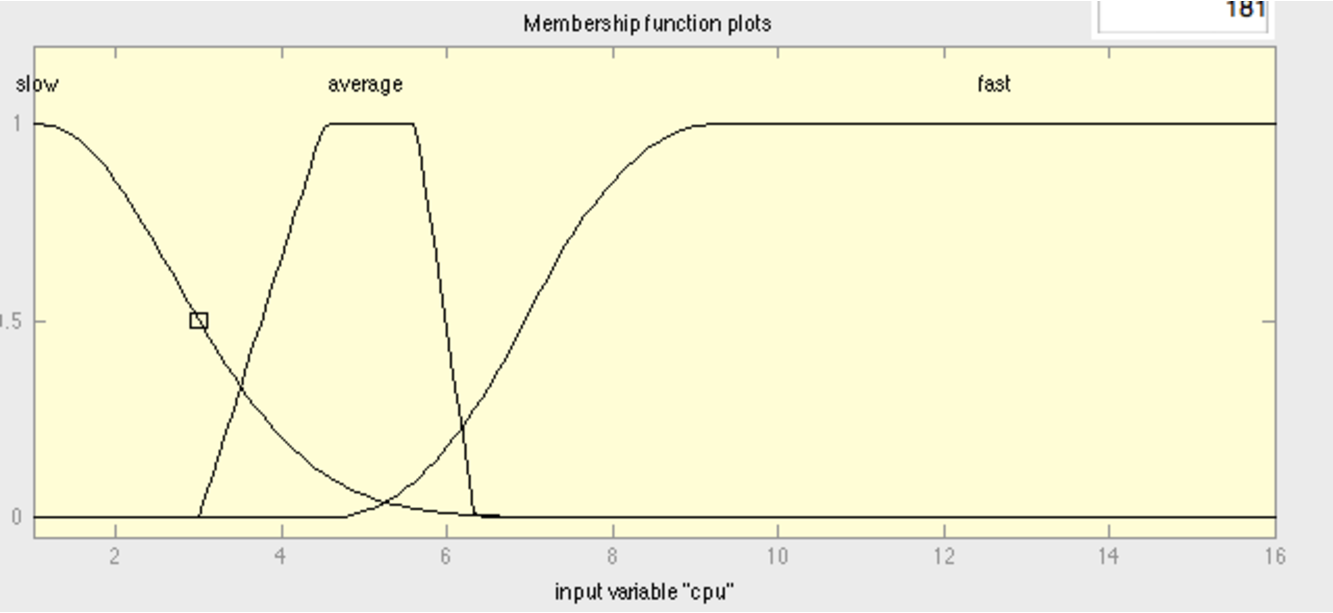
\includegraphics[width=5in]{cpulikely.pdf}
  \caption{对CPU建模的隶属度函数分布图}
  \label{fig:cpulikelyhood}
\end{figure}

分别对内存,网络进行建模,生成如下隶属度函数图
(\ref{fig:memlikelyhood}和\ref{fig:networklikelyhood})

\begin{figure}[h!]
  \centering
  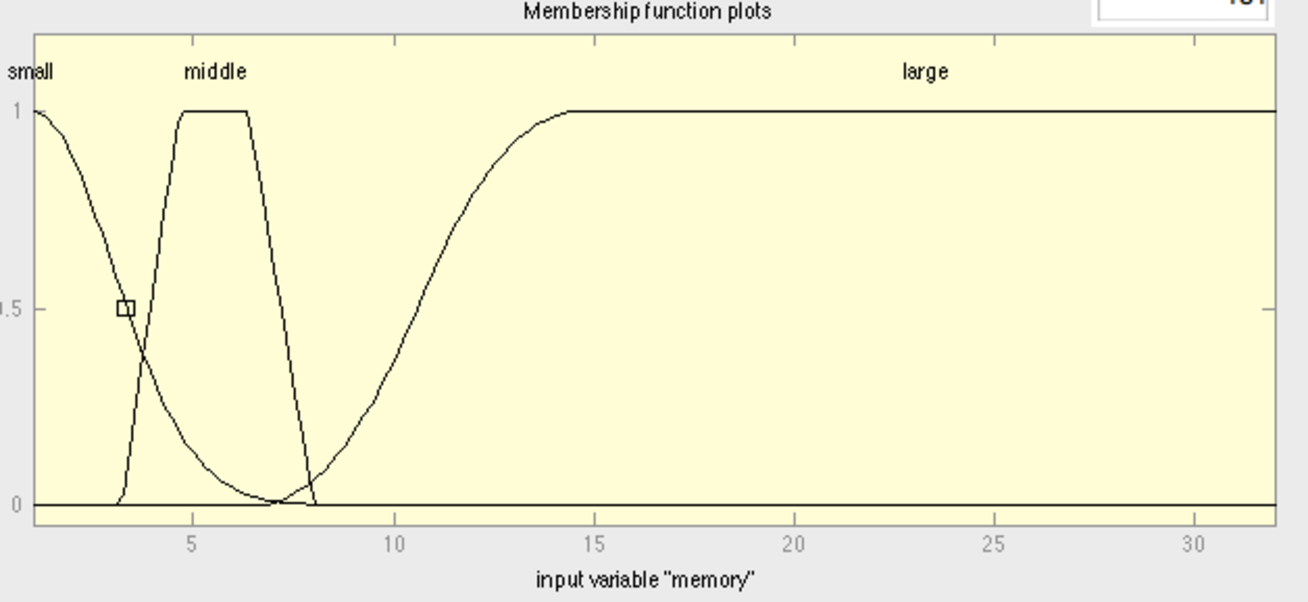
\includegraphics[width=5in]{memlikely.pdf}
  \caption{对内存建模的隶属度函数分布图}
  \label{fig:memlikelyhood}
\end{figure}

\begin{figure}[h!]
  \centering
  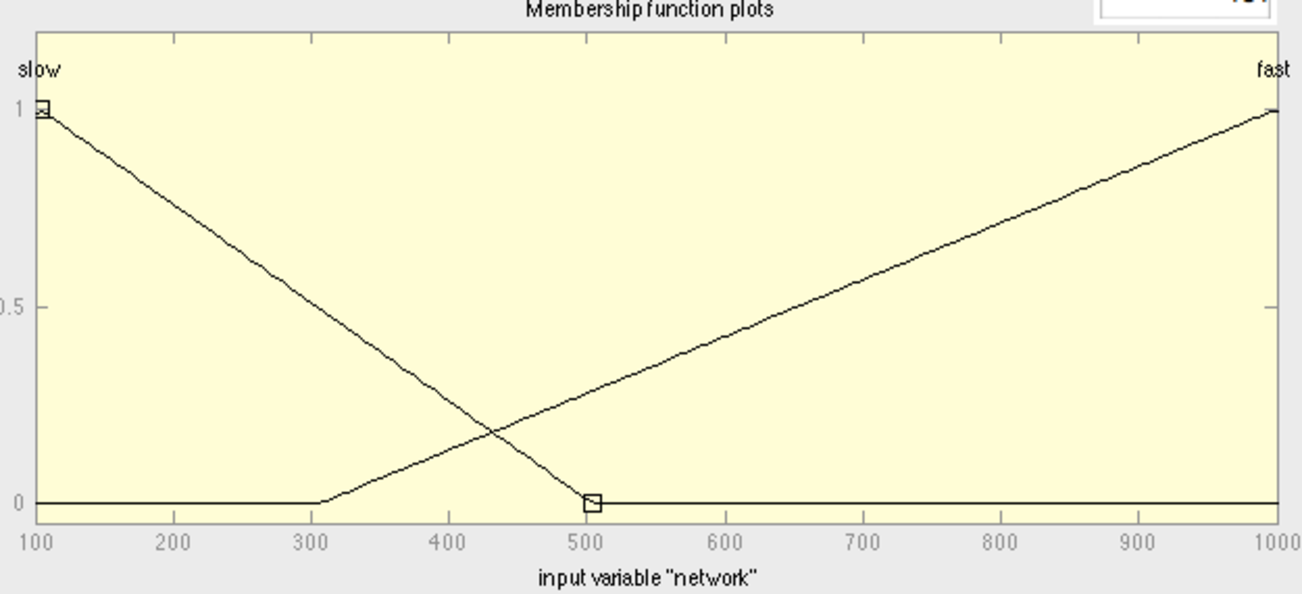
\includegraphics[width=5in]{networklikely.pdf}
  \caption{对网络建模的隶属度函数分布图}
  \label{fig:networklikelyhood}
\end{figure}

另一个输入来源就是执行的历史信息。在本文中我们认为任务执行的历史信息是
由多种原因造成的,特别是临时的错误,调度器的优先级等。因此它们并不适合
作为参数直接来影响模糊推理的结果,我们用它们作为最后的微调参数。

模糊逻辑的输出值为Hadoop配置参数中的值,我们在这里考虑了10个对系统性能
影响较大的参数\cite{hadoopconfexample, hadooptuning, speeduphadoop}.

\begin{table}[h!]\small
  \caption{模糊逻辑输出参数列表}
  \label{table:outputvars}
  \centering
  \begin{tabular}{|l c|}
    \hline
    \textit{参数名称} & \textit{取值范围} \\
    \hline
    io.sort.mb & 10-48-96-192-384-768 M \\
    \hline
    io.sort.factor & 10-40-80-120-240\\
    \hline
    io.sort.split.percent & 0-0.2-0.4-0.6-0.8-1.0\\
    \hline
    mapred.reduce.parallel.copies & 1-5-10-15-20\\
    \hline
    mapred.min.split.size & 64-128-256-512 M\\
    \hline
    mapred.tasktracker.reduce/map & \\
    .task.maximum & 1(1)-2(3)-3(5)-4(6)-5(9)\\
    \hline
    dfs.block.size & 64-128-256-512 M\\
    \hline
    mapred.map.tasks.speculative.execution & False -> True \\
    \hline
    mapred.reduce.task.speculative.execution & False -> True\\
    \hline
    mapred.job.shuffle.merge.percent & 0-0.2-0.4-0.6-0.8-1.0\\
    \hline
    mapred.job.shuffle.input.buffer.percent & 0-0.2-0.4-0.6-0.8-1.0\\
    \hline
  \end{tabular}
\end{table}

\subsubsection{模糊推理规则}
通过系统的调研Hadoop邮件列表中关于优化配置的参数和场景,我们为模糊算法
设定了合理的模糊规则。由于输入变量数目较多,输出变量更多,我们仅仅列出
其中一个模糊规则作为示例。\textit{io.sort.mb}指Hadoop的MapReduce任务执行过程中
对键值对进行排序时候可以使用的内存buffer的容量,单位为MB。
\textit{io.sort.mb}的隶属度集合如图\ref{fig:iomblikely}所示。

\begin{figure}[h!]
  \centering
  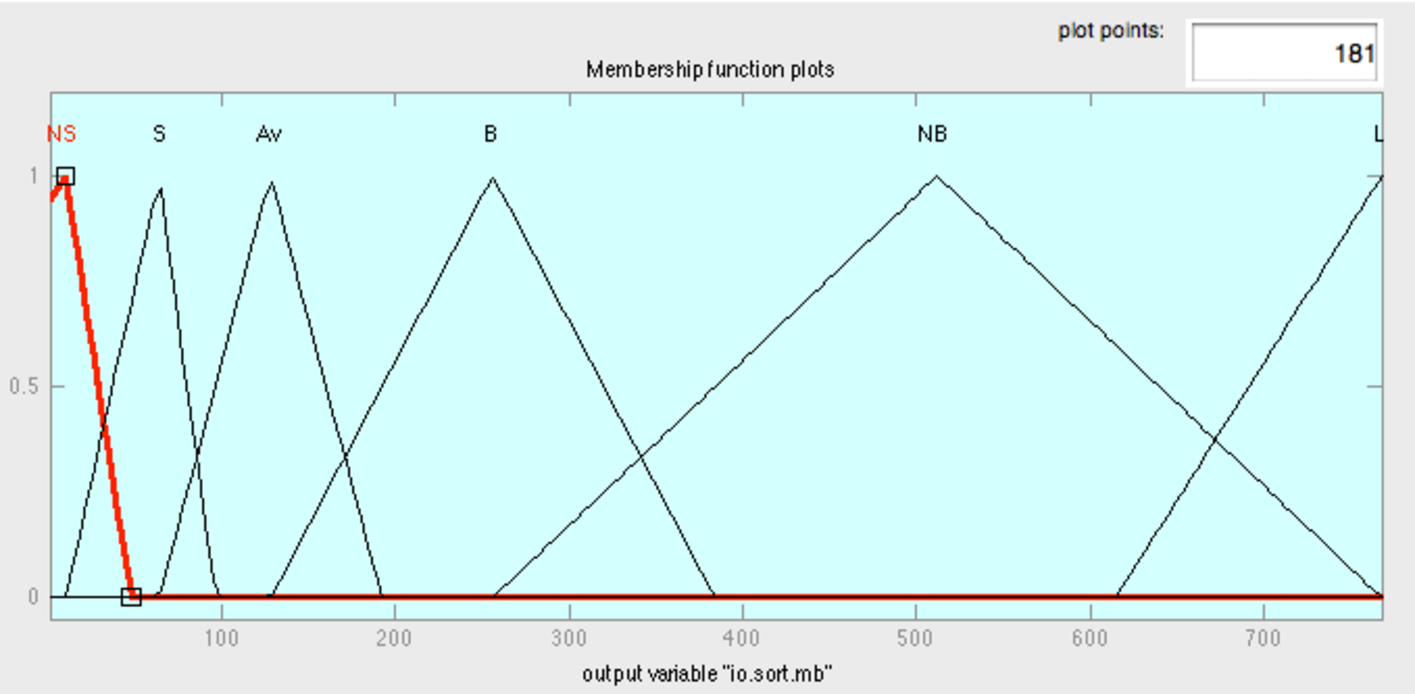
\includegraphics[width=5in]{iomblikeley.pdf}
  \caption{\textit{io.sort.mb}的隶属度函数}
  \label{fig:iomblikely}
\end{figure}

其对应的规则如图\ref{fig:iombrule}所示。

\begin{figure}[h!]
  \centering
  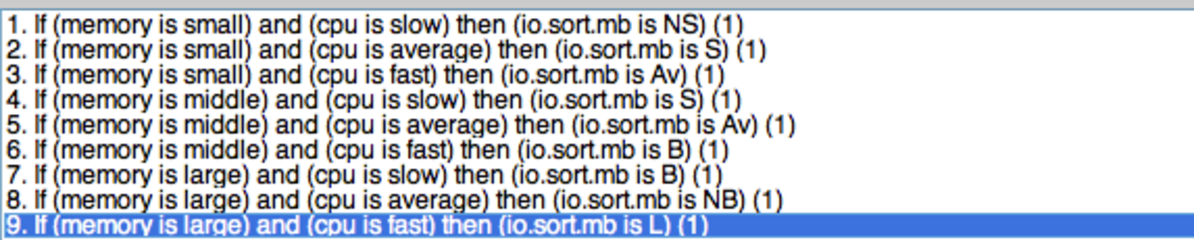
\includegraphics[width=5in]{iombrule.pdf}
  \caption{对\textit{io.sort.mb}的模糊规则表}
  \label{fig:iombrule}
\end{figure}

\section{实验和分析}
\subsection{Matlab仿真}
利用Matlab实现的模糊控制系统架构图(FIS)如下图\ref{fig:fis}所示。
\begin{figure}[h!]
  \centering
  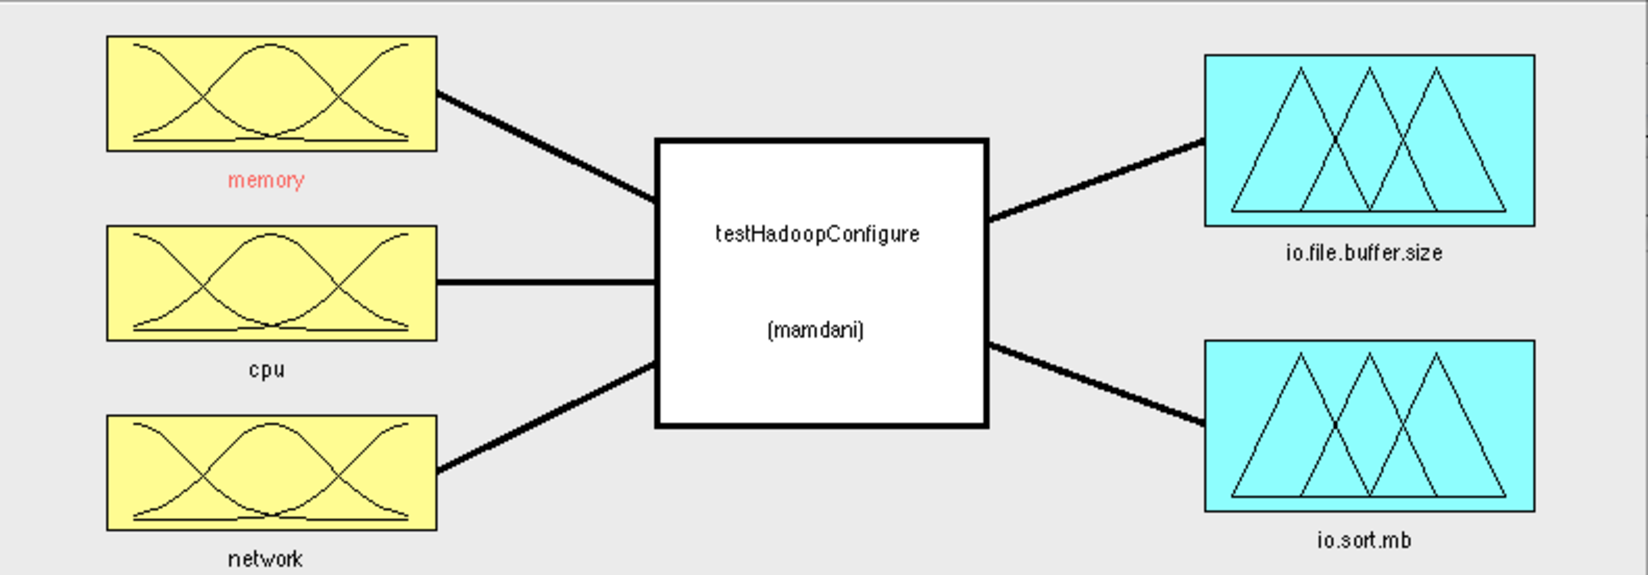
\includegraphics[width=5in]{fuzzyfis.pdf}
  \caption{系统的模糊控制系统总体图(仅列出了三个输入参数和两个输出参数)}
  \label{fig:fis}
\end{figure}
利用sufview可以得到\textit{io.sort.mb}和服务器中内存、CPU参数的输出曲
面,图\ref{fig:matlab}所示。
\begin{figure}[h!]
  \centering
  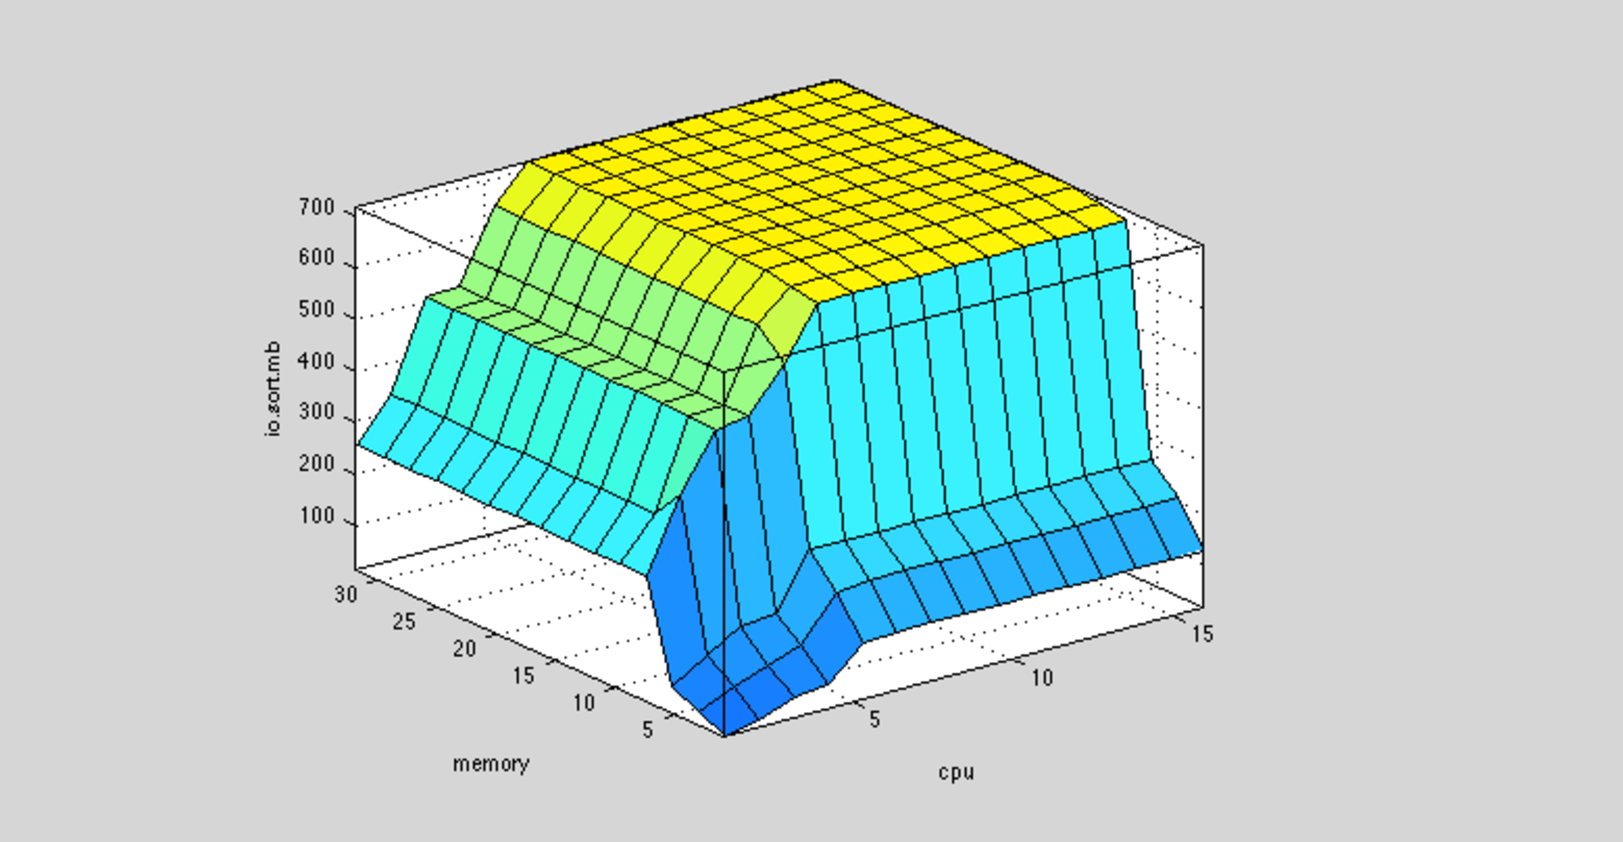
\includegraphics[width=5in]{matlab.pdf}
  \caption{参数\textit{io.sort.mb}的模糊规则输出三维示意图}
  \label{fig:matlab}
\end{figure}

\subsection{Hadoop集群实验}
通过修改Hadoop的源代码,我们为\textit{JobTracker}和
\textit{TaskTracker}实现了自动配置代码,通过检查历史运行数据来判断是否
需要重新配置,并将根据模糊逻辑生成的参数写入到本地配置文件中。

\subsubsection{同构环境实验}

所有的实验在一个由4台服务器构成的Hadoop集群上进行,其中3台slave节点,
一台master节点,所有节点性能配置如表\ref{table:machines}所示。

\begin{table}[h!]\small
  \caption{同构集群的节点参数}
  \label{table:machines}
  \centering
  \begin{tabular}{|c|c|}
    \hline
    \textit{属性} & \textit{参数} \\
    \hline
    CPU & Xeon W3530 2.53GHz\\
    \hline
    Memory & 6G 1066MHz ECC\\
    \hline
    Disk & 1T SATA Raid 1\\
    \hline
    Network & 100MB Ethernet\\
    \hline
  \end{tabular}
\end{table}

实验基于Hadoop发行版中自带的Terasort应用。使用默认配置参数运行该引用之后,再次使用自动化配置后得到的参数
运行Terasort,多次实验(每个实验执行10次)平均后比较性能。输入数据为25GB,最后结果如表\ref{table:tera1}所示。

\begin{table}[h!]\small
  \caption{运行25G Terasort所花费的时间}
  \label{table:tera1}
  \centering
  \begin{tabular}{|c|c|c|}
    \hline
    & \textit{Default} & \textit{Autoconfigured}\\
    \hline
    & 44min & 19min,40s\\
    Tera-Sort & &\\
    & 376maps, 16min & 94maps, 1min\\
    & 1reduce, 43min & 3reduce, 19min\\
    \hline
  \end{tabular}
\end{table}

采用默认配置的Hadoop集群运行一次任务需要2640s,
其中共运行了376个map任务共耗时960s,一个reduce任务,耗时2580秒。采用我
们的模糊推理得到的参数运行同一个任务只需要1180s,其中公允性了94个map任
务耗时60秒,3个reduce任务,耗时1140秒,加速比为2.23.此实验结果表明使用
模糊逻辑配置的工具能够得到较好的集群性能。


\subsubsection{异构环境实验}
通过人为降低集群中某一台服务器的内存,并且使其只启动一个CPU核来构
造异构的环境,该服务器的配置如下表\ref{table:m2}所示。

\begin{table}[h!]\small
  \caption{同构集群的节点参数}
  \label{table:m2}
  \centering
  \begin{tabular}{|c|c|}
    \hline
    \textit{属性} & \textit{参数} \\
    \hline
    CPU &  OneCore  2.53GHz\\
    \hline
    Memory & 2G 1066MHz ECC\\
    \hline
    Disk & 1T SATA Raid 1\\
    \hline
    Network & 100MB Ethernet\\
    \hline
  \end{tabular}
\end{table}

同样使用Terasort作为基准测试,并且和之前同构环境下测试时生成的
配置文件进行比较。执行10次后平均时间如表\ref{table:tera2}所示。

\begin{table}[h!]\small
  \caption{运行25G Terasort 同构和异构配置的性能对比}
  \label{table:tera2}
  \centering
  \begin{tabular}{|c|c|c|}
    \hline
    & \textit{homo-configured} & \textit{heter-configured}\\
    \hline
    & 33min & 27min\\
    Tera-Sort & &\\
    & 94maps, 11min & 94maps, 7min\\
    & 3reduce, 31min & 3reduces, 25min\\
    \hline
  \end{tabular}
\end{table}

结合表\ref{table:tera1}和\ref{table:tera2},我们可以得出结论,采用同构
环境下计算出来的结果来配置异构集群会使得集群性能降低,并且这个性能降低
(从19min到33min)远远超过了一台服务器性能折半带来的性能降低。这说明了在
异构环境下使用正确的参数配置的重要性。通过实验结果也可以看出来,采用异
构配置的集群其性能明显优于同构的配置参数。

\section{小结}
本研究使用模糊逻辑的方法对大规模部署的异构Hadoop集群进行参数
配置,并且通过试验证明了本方法能够明显的提高Hadoop集群中MapReduce任务
执行的速度。然而面临着不断出现的对系统反应时间有着更高要求的应用,
Hadoop和MapReduce模型本身的设计上的限制决定了其无法适用于这类应用。从
下一章开始,我们将介绍新型的分布式存储系统以及新的计算模型来进一步应对
实时应用的需求。
